\section{The Microcontroller}
\label{sec:TheMicrocontroller}

 Given the design requirements in section \ref{sec:RequirementsSpecification}, and the block diagram in section \ref{sec:TheSystem}. This includes all the functionality that is to be placed in the microcontroller. From here the next stage is to define the content of these blocks, and how they interact with each other. 
 
 The microcontroller is to establish an application programmer interface (API) to the P\&T driver placed in the FPGA. The microcontroller will also run the application that uses this interface in order to help the user achieve his/her goal, which is to control the spotlight.
 
 The program will be written in the C language, and it will be documented using task diagrams and state machines. 


% program structure
\subsection{Choice of Operating System}
\label{sec:ChoiceofOperatingSystem}

Why use freeRTOS
- The tool used in our semester
- real tome system

what are the alternatives? 
there are my own operating system but the options here are limited

Witch limitations does FreeRTOS give os 
- no messages, but events
- no binary semaphores 
- (handling floating point - whitch i have never tested)



\subsection{Program Structure}
\label{sec:ProgramStructure}

After the definition of the operating system, the next stage was to define the actual application that needs to be implemented. Given the block diagram of figure \ref{fig:TheSystemBlockDiagram}, the blocks that make up the system were already defined.

\subsubsection{Defining tasks}
\label{sec:DefiningTasks}
First step is to identify the tasks that make up the system. A good rule of thumb is to make a driver task for every piece of hardware that the system is to interact with. This idea is based on the Parallel criteria, which implies that things can be separated into different tasks if the functionality run independently and simultaneously, which indeed will be the case for a hardware driver.
However the UART0 driver that supports connection between the PC and micro controller, can send and receive data independently. Therefore this task is split up in to two tasks. A receive task, and a transmit task.
Doing so also have the advantage of reusability, for other applications requiring the same hardware. 

Now when all the hardware is taken care of, the only thing remaining is the application itself. The application should be able to handle commands given by the user. Commands could be "set coordinate pan, tilt", "run light-show \#2" and "set minimum velocity tilt". Since the entire application will consist of function calls, the main body of the application will take the shape of a kernel task that executes the functions defined in the function list shown in appendix 
\ref{sec:KernelInstructionList}. However by executing the command "run lightshow" it requires of the application to feed the P\&T driver with new target points once the previus target point has been reached. Considering that one still would like to send commands while running a light-show this will make two tasks based on the parallel criteria. The kernel Task and the light-show task.

Last but not least the application operates on the current position in order to handle a light-show. But gaining the current position requires pulling from the application. This task therefore makes the final task in the system based on the Periodical Criteria. 

The application must therefore consist of the following tasks:

Driver tasks:
\begin{itemize}[noitemsep]
	\item UART0\_rx\_task
	\item UART0\_tx\_task
	\item Joystick\_task
	\item SPI\_Master\_task
\end{itemize}

Application tasks:
\begin{itemize}[noitemsep]
	\item app\_kernel\_task
	\item app\_lightshow\_task
	\item app\_update\_current\_task
\end{itemize}	
	
\subsubsection{Connecting the tasks}
Now the tasks are to be linked together. This will happen in a structure so that every task that requires input from other tasks has one and only one queue to pull from. This is decried since the OS can pause the task while waiting for one queue. The UART tasks and the joystick tasks will both send commands to kernel via the application queue, and a shared state memory. The same goes for the connection between the kernel task and the light-show task. 

Each queue needs to be semaphore protected in order to prevent a race condition when reading an writing to the queue, but since freeRTOS handles who gets to use the queues, it must be safe to assume that such conditions is taken care of in the OS. 

The shared state memory (SSM), needs semaphore protection as well. Since the number of memory locations is relatively small (less then 64), combined with the fact that the critical section only consists of one read or write. the entire SSM will be handled by the same semaphore for simplicity. 

The tow application tasks app\_update\_current\_task and app\_kernel\_task will both be accessing the spi\_tx\_queue, but this will only be a problem if they wish to send multiple messages in context, which is not the case for this application. The same goes for the application\_queue. Here the send messages and events content will be independent from each other.  

Applying all these thoughts will result in the final application task diagram as shown in figure \ref{fig:applicaiton_task_diagram}. Now when the task diagram has been made, it is time to consider possible structural weaknesses such as deadlocks and handling of queues. 

% full dreas task diagram
\begin{figure}
	\centering
	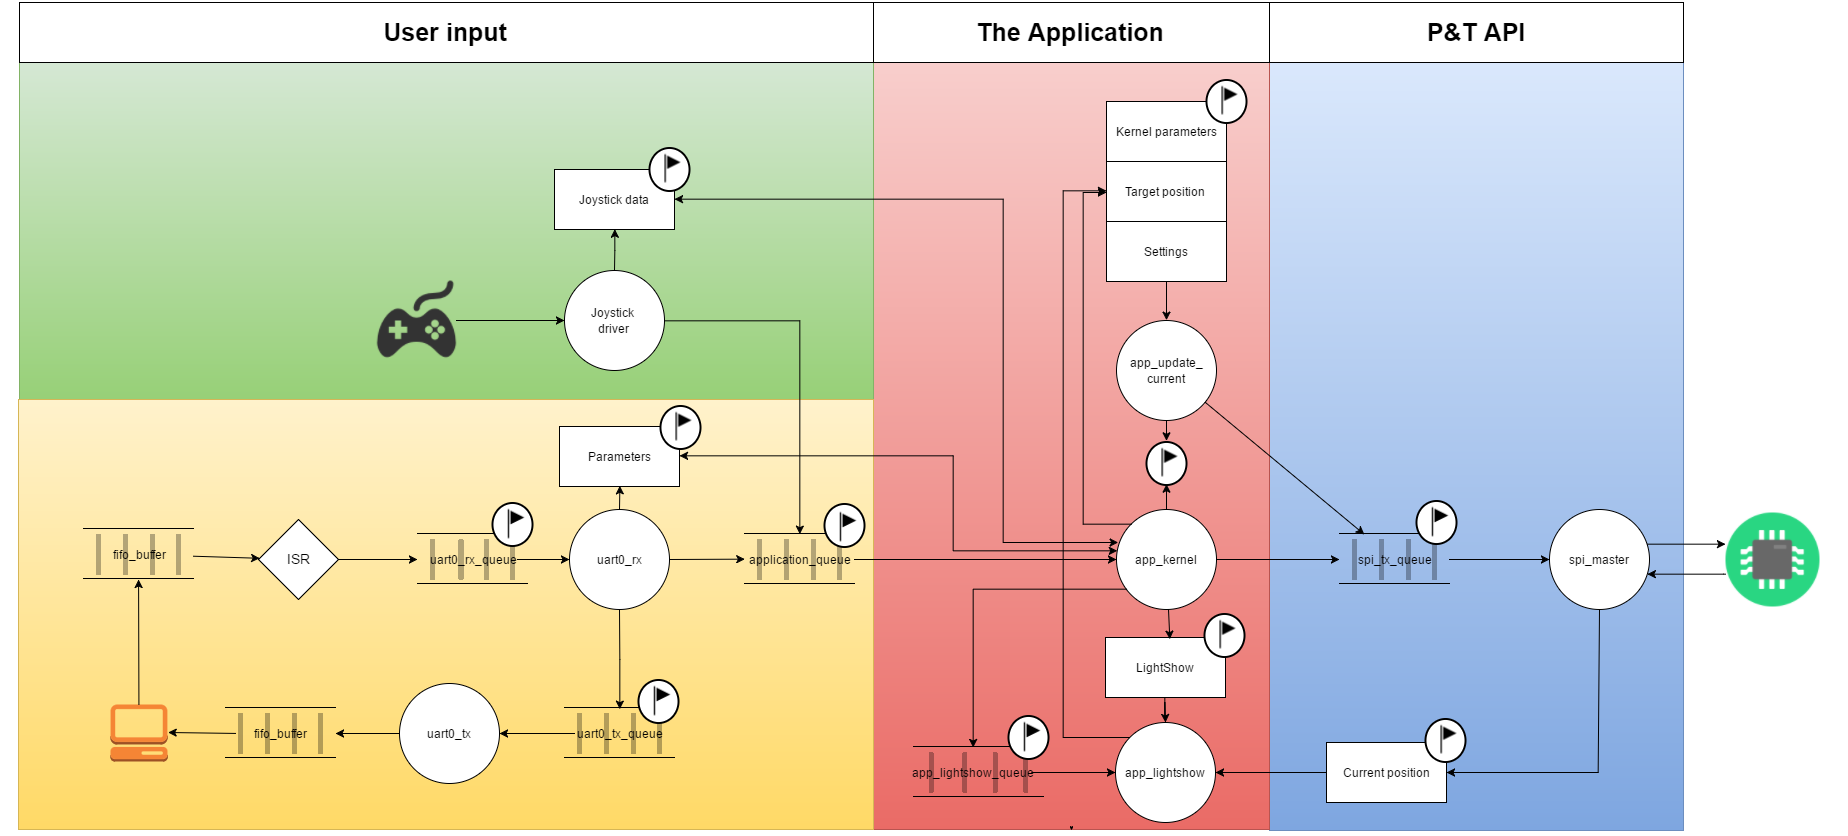
\includegraphics[scale= 0.4, angle = 90] {Billeder/microcontroller-Task-Diagram}
	\caption{The application task diagram}
	\label{fig:applicaiton_task_diagram}
\end{figure}

\subsection{The Application Programmer Interface}
\label{sec:TheApplicationProgrammerInterface}

what is this sorcery - and what will i achieve by using it
it is there to represent all the functionality available for each driver in the program.

where in the program will this be used

how will it be implemented 



\subsection{Event Queues and Shared State Memory}
\label{sec:EventQueuesandSharedStateMemory}

When operating with tasks, it should come as no surprise that it will be implemented as a state machine. This structure will operate in one state until a specific condition is met, from here the tasks will operate en ways defined by the new state. For this application the tasks will mostly switch states as they receive the correct events. In short an event is a number that the programmer has assigned a specific meaning to. It is therefor impotent for the application to know if it is reading an envent ore not.  In other words, if the sending task uses the queue for both user data and events, it will be impossible for the reviver to know, if the number 214 is to be interpreted as the value, or the event e.g "UPDATE\_DISPLAY". 


Suppose an event is an eight bit unsigned integer, and it is send to a task through a queue. It is imposible for the receiver task to know what data type it is, and who send it. It will therefore have to send extra information stating the data type in the shape of a header message. 
An alternative would splitting up the comunication in a event\_queue and a SSM buffer. Only events will go in the queue, and data will first be placed in the SSM and then an SSM\_READ event is send to the receiver task. Form here the reciever will read the data and set it to zero. 

It is possible to first send a header message telling what to do with the next message, however, this solution would not be particularly robust, since all it takes for the system to get lost is for one message to fail at either get send or received incorrectly. It will then go out of synchronization and header will be read as data and the other way around, and since this error only happens at rarely this error will be hard to debug. It is therefore preferred to keep the messages atomic, by using a queue and a SSM address. 
 










\subsection{Deadlock Protection}
\label{sec:DeadlockProtection}

A deadlock is when one or more process cannot proceed because some of the resources it need is held by another process. The two processes will "compete" with each other and neither of them will finish.
 
\begin{enumerate}[noitemsep]
	
	\item \textbf{Mutual exclusion} is the concept of making sure that two or more concurrent processes are not in their critical section at the same time. The critical section is a part of the program that cant be used by more than one process at the time.\\ If more than one process is in the same critical section at the same time errors are bound to happen.
	
	\item \textbf{Hold and wait} is when a process holds on to a resources and wait for the rest of the resources it needs.
	
	\item \textbf{no preemption} means that only the process that holds the resource can release it. If preemption is allowed, the program is able to take resources from a process and allocate it to another process.
	
	\item \textbf{Circular wait} is when one process is waiting for at resource that another process is has and the other process is waiting for a resource held by the first one. It could also be a chain of processes where every process needs a resource held by the next and the last one needs a resource held by the first.
	
\textbf{(add source XXXX)}
	
\end{enumerate}

All four conditions needs to hold true in order for a deadlock to occur. You can therefore provide a deadlock-free environment by avoiding one of the conditions. 

To avoid deadlocks in the system, the circular wait condition is removed via semaphores. This insures that deadlock cannot happen. In figure \ref{fig:Semaphore} a code example of how it is used.

\begin{figure}[h!]
\centering
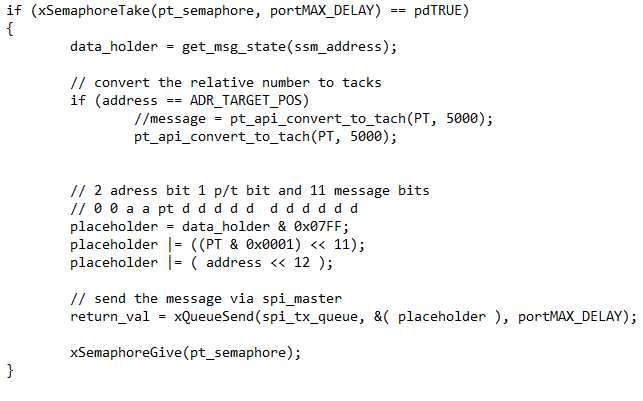
\includegraphics[scale=0.6]{Billeder/Micro_Controller/Semaphore_code_example.png}
\caption{ Semaphore code example }
\label{fig:Semaphore}
\end{figure}

First the process takes one semaphore. Then it takes another, do \textbf{SKRIV HVAD DEN GØR}. After that it releases the first semaphore and then the last. This insures that it has all the resources it needs to do its work and no deadlock is possible.













\subsection{SPI-Master}
\label{sec:SPIMaster}

The microcontroller have to share information with the FPGA, and according to the requirements mentioned in section \ref{sec:Primaryrequirements}, this communication has to happen using Serial Peripheral Interface (SPI). The protocol will operate as descriped in section \ref{sec:SPIcommunication}. It is therefore important that this link never will be a bottleneck for the system application. 

The requirements of the minimum bit-rate depends om what data that needs to be send, and how often it needs to send it. Since the PID-controller is placed in the FPGA, the application only needs to update the current position once every 5 ms, which is the minimal delay that freeRTOS can put on a task. 

The length of the messages send is defined by the driver placed in the FPGA. As described in section \ref{sec:Implementation} all messages will have the length of 14 bits. Updating both pan and tilt requires two messages. Concidering all other messeges but the main pulling sequence neglecteble relult in a total bitrate of:

\begin{equation}
Bitrate = \frac{
14 bit * 2	
}{
0.05s
} = 5.600 bit/sec 
\end{equation}

The Cortex M4 have a build in frescale spi module, that supports four different variations of spi, se appendix \ref{sec:CortexM4Datasheet}. However, by implementing the spi from scratch, it will give highest degree of control over the process, which is prefer in this project. 

% full dreasd task diagram
\begin{figure}
	\centering
	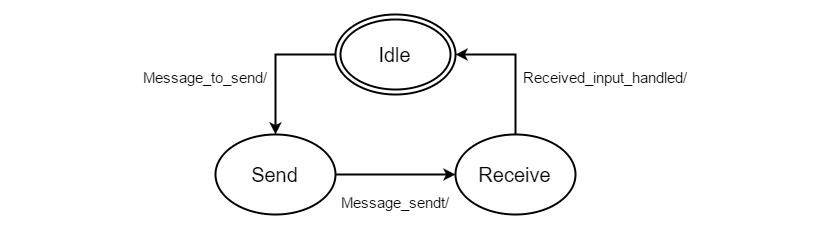
\includegraphics[scale = 0.7] {Billeder/SPI-master}
	\caption{The SPI-master state machine}
	\label{fig:SPI-master}
\end{figure}

The state machine for the task is illustrated in figure \ref{fig:SPI-master} is as simple at is gonna get. It consists of three states and is initiated waiting for a message to transmit from the spi\_tx\_queue. When a message is pulled from the queue it jumps to the send state, and after sending the message, the received message will be handled by the P\&T API in the Receive task. From here it will only switch back to the idle state if the API call was successful, else it will continue till it succeeds. 


\subsubsection{Performance Test} 
\label{sec:PerformanceTest}
After implementing the the SPI-master task in the final application the max bit-rate was tested by overloading the spi\_tx\_queue, and giving the SPI-master task High priority int the OS. This made the the task perform at maximum capacity. The measurements of the SPI connection can be seen in figure \ref{fig:HightPerformance}. Since it is able to transmit messages of 14 bots at 7.7 kHz the bitrate will be the product of these two values giving the result $107 kbit/sek$


\begin{figure}
	\centering
	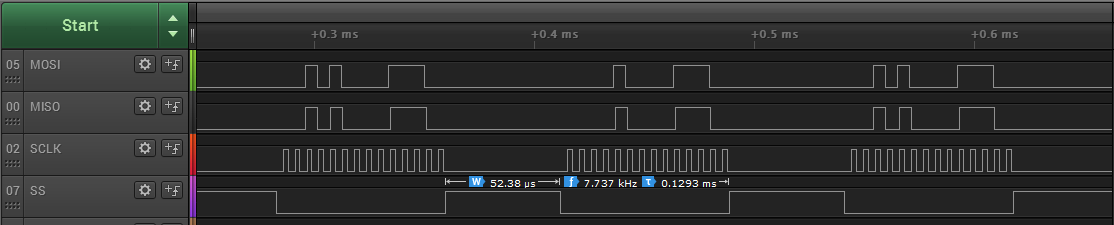
\includegraphics[scale = 0.7] {Billeder/HightPerformance}
	\caption{Shows the max performance of the SPI-Master task}
	\label{fig:HightPerformance}
\end{figure}
 

 





\subsection{The Application}
\label{sec:TheApplication}
Now when the interface for the application is set up, the only thing left is to program the actiual applocation , the 

\subsubsection{The Kernel task}


\begin{figure}[h]
	\centering
	\includegraphics[scale = 0.4] {Billeder/app-kernel-statemachine}
	\caption{The kernel state machine}
	\label{fig:KernelStateMachine}
\end{figure}
making the state mashine for the kernel-task

separating commands in groups depending on the number of parameters to use. 

the list of commands that will be supported (se the list on google drive XXXX)

\subsubsection{The light-show task}
making the state machine for the light-show-task








% summery 
\subsection{Overview}

The functionality of the system was meant as a fully dressed system containing all the features that would be needed while working with a real spotlight. However some of the secondary requirements cut from the final project.

\textbf{SKRIV GRUND SO DET IKKE LYDER SOM EN UNDSKYLDNING}


\textbf{The joystick:} Being able to control the spotlight via a PS2 controller is a secondary requirement. A working driver was made but the corresponding API was not. This meant that this feature was not implemented. This is not a problem as it is possible to control the system via the a PC though the UART.


\textbf{Position vs given coordinates:} The input from the P\&T system is tachs(falling and rising edges from the Hall effect sensors). This correspond to an orientation on a sphere. As the target for the spotlight is a flat surface, some conversions is needed in order to translate the desired position on the scene to an amount of tachs. The conversion takes place in \textbf{HVOR SKER DET?}.


\textbf{Following a walking person:} The system is not build with the option to change the speed, based on user input, between points. This means that rather than following a walking person, the system points at different points of the stage.


This is the functions that did not make it to the implementation

\begin{enumerate}[noitemsep]
	
	\item PS2 controller and its corresponding api
	
	\item Calculating the tack-position from the relative coordinates given by the application  
	
	

\end{enumerate}